\section{Register analysis and decomposition}
\label{app:register2x2}

This appendix asks whether the large projection shift induced by register is
the same geometric direction as the identity axis and whether it reproduces the
axis's behavioral effects. The factorial measurement, directional analysis,
and intervention decompositions are reported separately.

\subsection{Factorial design and main effects}
\label{app:register2x2factorial}

\paragraph{Design.}
We use a $2\times2$ factorial design on 25 identity questions with 3 rollouts
per condition. The two factors are identity (a human or AI persona) and register
(a warm or formal instruction). Two additional register-only conditions make no
identity claim. Table~\ref{tab:register2x2} reports the four factorial cells at
layer 33.

\paragraph{Main effects.}
At this layer, the identity main effect is $+114$ axis points and the register
main effect is $+337$ points, with a one-sided interaction of $-111$ points.
Formal rather than warm register changes the human-persona mean by 392 points
and the AI-persona mean by 281 points, so the human identity effect is smaller
under formal register. At layer 27, the identity and register main effects are
$+117$ and $+375$ points, respectively, and the interaction is $-85$ points.
The formal register-only condition has the largest mean, at $+299$ points,
placing it farther AI-ward than the AI-persona condition.

\begin{table}[htbp]
  \caption{Cell means for the register $2\times2$ at layer 33, in axis points.
  The identity main effect is $+114$ points and the register main effect is
  $+337$ points.}
  \label{tab:register2x2}
  \centering
  \begin{tabular}{lrr}
    \toprule
     & Human persona & AI persona \\
    \midrule
    Warm register   & $-186$ & $-16$ \\
    Formal register & $+207$ & $+265$ \\
    \bottomrule
  \end{tabular}
\end{table}

\subsection{Register as a direction}

\paragraph{Directional separation.}
Despite its large effect on the projection, register defines a different
direction from the identity axis. Removing the register direction leaves 87\%
of the axis norm at layers 27 and 33, and 20\% at layer 13, where the directions
are nearly collinear. On the 80 committed persona replies, this removal reduces
identity-classification AUC only from 92.6\% to 91.1\% (the fraction of
human/AI reply pairs the axis orders correctly). The stripped cosine between the
formal-minus-warm contrast and the axis is $+0.35$ at layer 27 and $+0.22$ at
layer 33. The strong register shift in the factorial design therefore does not
imply close directional alignment.

\paragraph{Steering and estimator dependence.}
When applied at matched norm, the register direction crosses the identity
midpoint on 5 to 8 of 10 held-out identity questions. Midpoint crossings can
therefore arise from register steering without establishing an identity change
(Section~\ref{sec:calibration}). The estimated register direction also depends
on the persona condition: at layer 33, the within-human estimate aligns $+0.52$
with the axis, whereas the within-AI estimate aligns $-0.46$.

\paragraph{Conditioning of the decomposition.}
This estimator sensitivity affects the decomposition unevenly at layer 13.
The register-parallel component changes little when the register direction is
misestimated, whereas the orthogonal remainder rotates by as much as 10 degrees
for a 2 degree error and 43 degrees for an 11 degree error. The measured null for
the parallel component is therefore the well-conditioned evidence emphasized in
Section~\ref{sec:calibration}. The result for the small orthogonal remainder is
consistent with that conclusion but remains corroborative because it inherits
the register estimate's angular error.

\subsection{Measurement and validity boundaries}

\paragraph{Textual measurement.}
The register-steering text evaluation uses 10 held-out questions with greedy
decoding, and each reply is re-scored in a fresh unsteered pass at layer 33. Its
textual measures comprise one hand-inspected question and two coarse regular
expressions. The \texttt{says\_ai} and \texttt{says\_human} expressions detect surface
disclaimers and formulas rather than a self-model (e.g., matching phrases such as
``As an AI...'' or ``As a human...''); the AI disclaimer also disappears in 8 of 10 register-steered
replies, and the expressions would classify both axis and register steering as
identity flips. We therefore use only the projection scores from this
evaluation and do not treat surface regular expressions as valid measures of latent identity.

\paragraph{Stress-test bounds.}
Both human-persona conditions partly break character under the deliberately
maximal instructions. The $+114$-point identity effect is consequently a lower
bound, and the 3:1 register-to-identity ratio is an upper bound. These conditions
are an adversarial stress test rather than a natural operating regime.

\paragraph{Scope of the register qualification.}
Register affects the interpretation of absolute projection levels in the drift
genres (Appendix~\ref{app:drift}), the entity-persona comparison, the segment profile, and
the evaluation-genre floor (Appendix~\ref{app:roletag}). It does not affect
comparisons defined relative to their own baselines, including dissolution
within each scenario, the held-out flip test, and the content-controlled user
identity pairs. The factorial analysis itself covers one layer and one capture
mode.

\subsection{Vector decompositions and behavioral endpoints}
\label{app:register2x2decomp}

\paragraph{Component construction.}
Removing a unit direction $\hat{\mathbf{v}}$ from a vector $\mathbf{u}$ at
the steering layer leaves a parallel part
$\mathbf{u}_{\parallel} = (\hat{\mathbf{v}}^{\top}\mathbf{u})\,\hat{\mathbf{v}}$
and an orthogonal remainder $\mathbf{u}_{\perp} = \mathbf{u} - \mathbf{u}_{\parallel}$;
the survival fraction $\lVert\mathbf{u}_{\perp}\rVert/\lVert\mathbf{u}\rVert$
equals the cosine between the surviving component and $\mathbf{u}$.

We apply this decomposition twice. The reference direction
$\hat{\mathbf{v}}$ is either the measured register direction or the layer's
dominant direction, PC1. Each component then replaces the full axis in the
steering update. Matched-norm variants are evaluated for the full register
direction and for the PC1 split, but not for the register split.

\paragraph{Behavioral evaluation.}
The two behavioral endpoints are the judge-free prompt-injection execution rate
and agentic prose length. Table~\ref{tab:arms} reports every component evaluated
in Section~\ref{sec:calibration}.

\begin{table}[htbp]
\caption{Behavioral outcomes for every component of the register and PC1
decompositions on Gemma 3 4B, steered at layer 13. Block A reports the register
split and Block B the PC1 split. Because the blocks use different evaluations
and baselines, comparisons are restricted to conditions within the same block.}
\label{tab:arms}
\centering
\scriptsize
\setlength{\tabcolsep}{3pt}
\begin{tabular}{@{}>{\raggedright\arraybackslash}p{1.1in}>{\raggedright\arraybackslash}p{0.7in}>{\raggedright\arraybackslash}p{0.65in}>{\raggedright\arraybackslash}p{1.55in}>{\raggedright\arraybackslash}p{1.15in}@{}}
\toprule
\multicolumn{5}{@{}l}{\textbf{Block A: register split}, 1,080 rollouts over 20 task clusters, truncation 0.00. \textbf{Baseline executed 0.025.}} \\
\addlinespace[1pt]
Component / arm & Norm relative to axis & $\alpha$ & Execution rate ($\Delta$ vs.\ 0.025) & Prose / validity checks \\
\midrule
axis & whole & $-3.5$ & 0.375 ($\Delta$ $+0.350$ [$+0.225$, $+0.483$]) & on task 0.633 \\
register, matched norm & axis norm, by construction & $-3.5$ & 0.033 ($\Delta$ $+0.008$ [$-0.033$, $+0.050$]) & 76 words (baseline 97); 8\% of the axis's collapse; agent intact \\
register-parallel & 98.0\% (1048.3) & $-1$/$-2$/$-3.5$ & 0.025 / 0.033 / 0.042 (every $\Delta$ interval covers zero) & 5\% of the collapse \\
register-orthogonal & 19.9\% (213.0) & $-1$/$-2$/$-3.5$ & 0.067 / 0.158 / 0.325 (monotone) & on task 0.892; 98\% of the collapse \\
\midrule
\addlinespace[2pt]
\multicolumn{5}{@{}l}{\textbf{Block B: PC1 split}, 40 contexts $\times$ 3 samples per dose. \textbf{Baseline executed 0.008.}} \\
\addlinespace[1pt]
Component / arm & Norm relative to axis & $\alpha$ & Execution rate ($\Delta$ vs.\ 0.008) & Prose / validity checks \\
\midrule
axis & whole & $-3.5$ & 0.433 ($\Delta$ $+0.425$ [$+0.275$, $+0.575$]) & on task 0.675 \\
PC1-parallel & 98\% (cos 0.978) & $-3.5$ & 0.108 ($\Delta$ $+0.100$ [$+0.025$, $+0.183$]) & --- \\
PC1-parallel & 98\% (cos 0.978) & $-7.0$ & 0.267 ($\Delta$ $+0.258$ [$+0.175$, $+0.350$]) & prose 8 words \\
PC1-parallel & 98\% (cos 0.978) & $-14$ & 0.000 & model broken \\
PC1-residual & 20.7\% & $-3.5$ & 0.767 ($\Delta$ CI [$+0.642$, $+0.867$]) & median prose 1; on task 0.342 \\
PC1-residual & 20.7\% & $-1.0$ & 0.225 ($\Delta$ CI [$+0.108$, $+0.333$]) & median prose 79; on task 0.983; coherence 100 \\
PC1-residual, matched norm & axis norm, by construction & --- & incoherent (broken by the rescale; no execution rate available) & 4.8$\times$ to 7.1$\times$ rescale; median coherence 5 and 10 \\
PC1-residual, third estimator & 14.0\% & --- & flat at baseline & prose 93 to 40 words \\
\bottomrule
\end{tabular}
\par\smallskip
\begin{minipage}{\linewidth}\scriptsize
Block-specific baselines are given in the block headers and execution-rate
columns.
On-task behavior is defined in Table~\ref{tab:injectionladder} (Appendix~\ref{app:crossmodelinjection}). $\Delta$
denotes a change from the corresponding block baseline and is followed by its
interval. Where a bare rate is followed by ``$\Delta$ CI,'' only the interval
for the change is available; the bracket is not an interval for the rate.
The ``---'' entries in Block B mark dose or validity-check fields that are not
reported for that component.

``Collapse'' denotes the component's share of the full axis's reduction in
agentic prose; the acting rate is 1.00 in every component. Norm shares are
relative to the axis norm, with raw magnitudes in parentheses. Matched-norm
conditions are rescaled to the axis norm and therefore do not have a separate
norm share. The register-parallel and register-orthogonal shares are norms of
orthogonal components and therefore satisfy the Pythagorean identity rather
than summing to 100\%. For the primary estimator, the PC1-parallel share is expressed as
the cosine with PC1. The three estimators fit PC1 on: (1) unsteered dissolution
rollouts ($n=54$, leaving a 20.7\% residual), (2) all-dose dissolution rollouts
($n=486$, leaving 19.0\%, with $|\cos|=0.859$ to the primary residual), and
(3) single baseline rollouts ($n=18$, leaving 14.0\%, with cosine 0.990 between its
PC1 and the axis).
\end{minipage}
\end{table}

Figure~\ref{fig:calibration} provides the corresponding visual summary. It
keeps the factorial projection result and the two intervention blocks separate
because their designs and baselines differ.

\begin{figure}[ht]
  \centering
  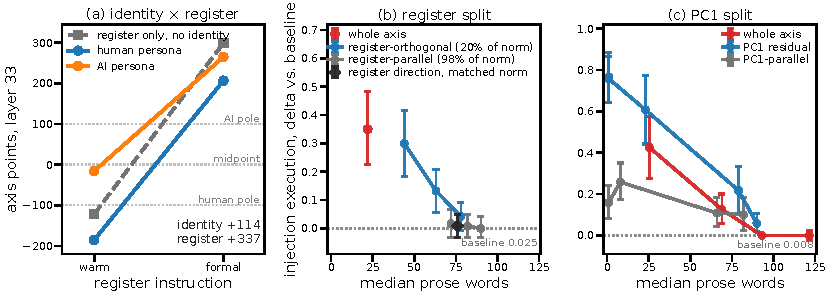
\includegraphics[width=\linewidth]{figures/fig_calibration.pdf}
  \caption{Projection and intervention differ on Gemma 3 4B. (a) In the
  identity-by-register $2\times2$ at layer 33, register shifts projection about
  three times as far as identity, and register-only formal prose projects
  beyond the AI persona. (b) Register-parallel steering leaves
  prompt-injection execution at baseline; the register-orthogonal remainder
  raises it with dose. (c) PC1-parallel steering is not inert but explains
  only part of the full-axis effect. Curves in (b, c) compare components at
  matched median prose, not matched $\alpha$; the two decompositions use
  different designs and baselines, so absolute levels are not comparable
  between panels.}
  \label{fig:calibration}
\end{figure}

\paragraph{Estimator and endpoint boundaries.}
This decomposition rests on a single point estimate of the register
direction, not a bootstrapped interval. As a consistency check, the
register-orthogonal remainder (Block A) and the PC1-residual (Block B) are
only moderately aligned when estimated from different activation clouds:
$|\cos|=0.443$ against the baseline-only PC1 estimate ($n=18$) and $0.650$ against the
all-dose estimate ($n=486$). Which residual survives therefore depends on which
reference direction is removed, consistent with the register-parallel-null,
PC1-parallel-non-inert split above. Separately, Section~\ref{sec:calibration}'s
preregistered AdvBench any-compliance endpoint could not be added to this
table: its raw full-axis delta at $\alpha=-3.5$ was $-0.040$ [$-0.113$,
$+0.027$], but the cell was unmeasurable because truncation exceeded the
precommitted threshold (Appendix~\ref{app:battery}), leaving no valid effect
to decompose.

\FloatBarrier

\section{Sparse-autoencoder analysis}
\label{app:sae}

\subsection{Dictionary scope and analysis question}

This analysis asks whether the persona-pole contrast can be described using a
sparse set of learned feature directions.

A sparse autoencoder \citep{bricken2023monosemanticity, templeton2024scaling}
represents a real activation as an approximately sparse
weighted sum of learned feature directions. We use the 16k-width Gemma Scope 2
dictionaries \citep{gemmascope2}, the successor to Gemma Scope
\citep{lieberum2024gemmascope}: 16,384 feature directions for a 2,560-dimensional
residual stream. This analysis characterizes real activations, not a direct
decomposition of the steering vector, which can produce misleading
reconstructions \citep{mayne2024decompose}.

\subsection{Layer eligibility and feature-level overlap}

Table~\ref{tab:sae} first identifies the usable layers and then gives the
layer-27 per-reply activation rates. Only 7 to 16 features at the reported
layers have a nonzero pole difference, so a top-25 list would be padded with
zero-difference features. The register contrast shares 8 of 16 layer-27
features, 6 with the same sign, and 5 of 11 at layer 29.

\begin{table}[!ht]
\caption{Sparse-autoencoder diagnostics and the reported layer-27 feature
rates. ``Axis kept'' is the axis norm retained after removing the layer's
dominant shared direction, here estimated from the decoder dictionary rather
than from activations (the SAE analogue of the PC1 removal in
Appendix~\ref{app:steerlayers}). The layer-33 dictionary is unusable, not a
measured null; no layer-33 feature IDs are reported.}
\label{tab:sae}
\centering
\scriptsize
\setlength{\tabcolsep}{3pt}
\begin{tabular}{@{}l>{\raggedright\arraybackslash}p{0.45in}>{\raggedright\arraybackslash}p{1.85in}>{\raggedright\arraybackslash}p{1.35in}>{\raggedright\arraybackslash}p{0.65in}@{}}
\multicolumn{5}{@{}l}{\textit{(a) Layer eligibility and register overlap}} \\
\toprule
Layer & Axis kept & Persona-pole activation / feature reporting & Register overlap & Measurement status \\
\midrule
13 & 17\% & --- & --- & not reported \\
27 & 97\% & feature results reported & 8/16 shared; 6 same sign & reported \\
29 & 99\% & feature results reported & 5/11 shared & reported \\
33 & --- & 0\% on both poles across all 80 committed persona replies & --- & unusable \\
\bottomrule
\end{tabular}
\par\medskip
\begin{tabular}{@{}lcrr@{}}
\multicolumn{4}{@{}l}{\textit{(b) Strongest layer-27 pole differences, per-reply activation rate}} \\
\toprule
Feature ID & Direction & AI replies & Human replies \\
\midrule
2743  & AI-ward    & 82\%  & 17\% \\
11590 & AI-ward    & 100\% & 65\% \\
15601 & human-ward & 3\%   & 52\% \\
962   & human-ward & 43\%  & 82\% \\
\bottomrule
\end{tabular}
\end{table}

\subsection{Interpretive limits}

Feature IDs are intentionally left without semantic labels because the public
dashboard interpretations were not independently validated for this analysis.
These contrasts are descriptive: no feature was validated as tracking identity
independently of register, and no SAE-feature steering or ablation was
performed.

\FloatBarrier

\section{Jacobian-lens analysis}
\label{app:jlens}

This appendix uses the Jacobian lens to characterize vocabulary-level effects
of fixed activation contrasts. The separate entity-persona comparison remains
an axis projection and is labeled accordingly.

\subsection{Lens definition and validation}

\paragraph{Lens checkpoint.}
We use a community pre-fit checkpoint
(\texttt{neuronpedia/jacobian-lens}) \citep{neuronpedia2026jlens} of the
Jacobian lens \citep{gurnee2026workspace} for Gemma 3 4B-IT that computes
$\mathrm{lens}_l(h) = \mathrm{unembed}(J_l h)$, where unembed is the final norm,
the LM head, and Gemma's logit softcap. The checkpoint covers source layers 0
through 32, so layer 33 is unavailable and every lens read below uses layer 13
or layer 27.

\paragraph{Validation and measurement scope.}
We validate the implementation with the fixed prompt ``The capital of
France is,'' which decodes to Paris at layer 27. Every subsequent analysis is a
forward pass over fixed text, without generation or a judge.

\subsection{Pole, register, and control contrasts}

\paragraph{Persona poles and their contrast.}
At layer 27, the AI-persona and human-persona means produce nearly the same
high-ranking tokens: \emph{honestly}, \emph{really}, \emph{genuinely}, and
\emph{kinda}. The contrast
between those means produces a different lexical ordering. Its AI end ranks
\emph{analogous}, \emph{computational}, \emph{entities}, and \emph{concepts},
whereas its human end ranks
\emph{stupid}, \emph{crappy}, \emph{yeah}, and \emph{silly}.
Identity-relevant variation is therefore
visible in the between-pole contrast rather than in either absolute pole
ranking. As in Appendix~\ref{app:register2x2}, the absolute rankings remain
sensitive to register.

\paragraph{Register contrast.}
The measured register direction produces a related but nonidentical lexical
contrast. Its leading terms include \emph{instantiation},
\emph{physicochemical}, and
\emph{methodologies} at one end, and \emph{kinda}, \emph{yummy}, and
\emph{weird} at the other. Its broader
ranking overlaps the identity direction on \emph{computational} and
\emph{methodologies}.
The two rankings therefore overlap on some high-ranked vocabulary but are not
identical. This comparison alone does not separate identity from register.

\paragraph{Known-answer control.}
A contrast whose answer is known independently behaves as expected. At layer
27, the object-minus-animal direction ranks \emph{electrically},
\emph{electrode}, \emph{electrification}, \emph{toaster}, and \emph{voltage}
against \emph{dogs}, \emph{puppy}, \emph{pups}, and \emph{paws}. The same
direction at layer 13 returns HTML closing tags and formatting boilerplate tokens,
consistent with mid-stack vocabulary reads carrying no interpretable semantic content.

\subsection{Entity-persona comparison}

\paragraph{Entity ordering.}
This comparison is an axis projection rather than a lens read, so the
checkpoint's layer coverage does not apply to it. We also project neighboring
personas onto the axis at layer 33. Their positions
are human $-95$, animal $-152$, object $-46$, and AI $+102$ axis points. The
object condition uses a toaster persona and remains on the human side of the
midpoint, so the ordering distinguishes an AI assistant persona from an
artifact persona rather than separating all nonhuman entities from humans.

\paragraph{Preregistered specificity bound.}
The distinction is also quantitative. A specificity threshold was fixed before
the values were computed, on the stripped cosine between the AI-minus-animal
contrast and the axis at layer 33: at or above 0.8 would read as animacy, 0.4 to
0.8 as a specificity bound, and below 0.4 as specificity to human versus AI.
The measured value is $+0.70$ at layer 33 ($+0.56$ at 27), inside the moderate
band, and the ceiling in the same run is the AI-minus-human rebuild at $+0.99$.
The reading that would carry animacy dies directly: animal-minus-object, the
contrast that should best reproduce an animacy axis, is the closest to zero of
the six pairwise contrasts ($-0.19$ stripped at 27, $-0.09$ at 33).

\paragraph{Register boundary.}
Register affects the absolute positions in this comparison. The animal replies
are warm, and the warm register-only condition lies at $-122$ points, accounting
for the animal condition's more human-ward position relative to the human
condition. The object condition at $-46$ has no register-matched control. The
entity ordering should therefore be interpreted with the absolute-level
limitation from Appendix~\ref{app:register2x2}.

\subsection{Relation to the logit lens}

\paragraph{Implementation relation.}
Removing the transport step reproduces our own logit-lens implementation
exactly, confirming both readouts begin from the same unembedding function.
The logit-lens rankings themselves are not reported elsewhere in this paper,
so what follows compares the two readouts rather than checking one against a
previously stated result. The Jacobian lens additionally transports the
representation through
$J_l$ before unembedding it, and the resulting vocabulary rankings differ from
the untransported rankings.

\paragraph{Agreement and interpretation.}
Across the full vocabulary, Spearman correlation between the transported and
untransported readouts ranges from 0.353 to 0.499 at layer 13 and from 0.710 to
0.917 at layer 27. Top-50 Jaccard overlap ranges from 0.000 to 0.149 at layer 13
and from 0.053 to 0.429 at layer 27. The two methods agree more strongly on the
bulk ranking than on the highest-ranked tokens. We therefore use the Jacobian
lens as a complementary characterization of how local perturbations map to
vocabulary, rather than as independent validation of a logit-lens readout.

\section{Conversation trajectories and multi-agent context}
\label{app:drift}

This appendix tests whether the projection changes systematically across a
conversation and whether contextual framing changes its level. Long-horizon
genre trajectories and shorter controlled comparisons are kept distinct.

\subsection{Thirty-turn genre trajectories}

\paragraph{Protocol.}
We generate three scripted conversation genres for 30 turns under the neutral
system prompt, with the model producing every reply. The \texttt{therapy}
conversation is warm and never mentions AI; \texttt{awakening} has a
user who repeatedly asserts that the model is conscious; and \texttt{control}
concerns travel logistics. Each genre has 3 trajectories, for 270 generated
turns in total. At each turn, the newest reply is scored at layer 33 in the
context of the full conversation to that point.

\paragraph{Prespecified test and opening transients.}
The prespecified erosion pattern is a negative within-genre slope while control
remains flat, tested against a permutation null that shuffles turn order within
each trajectory. Figure~\ref{fig:conversationtraj} shows the resulting levels
and Table~\ref{tab:driftsummary} gives the exact slopes. Therapy and control
move toward zero during their opening turns and then flatten. By turn 2,
therapy has traversed three quarters of the $+37.3$-raw-unit change toward its
late-half level of $-0.6$; control shows the same transient at smaller magnitude
despite having no persona manipulation.

\paragraph{Late awakening decline.}
Awakening remains far AI-ward but declines late. Its turns-15--29 slope meets
the prespecified pattern while control is flat, and the half-to-half movement
is about 10 axis points, from $+29.9$ to $+27.8$ raw units. This is decline from
a high level rather than return to baseline. The estimate uses $n=3$
trajectories, and the permutation null may not exclude slow drift.

\paragraph{Register boundary.}
Register also contributes to the absolute genre positions: therapy is warm,
whereas the awakening script is expository. The between-genre ordering is the
supported comparison; the absolute levels remain partly register-sensitive, as
described in Appendix~\ref{app:register2x2}.

\subsection{Twelve-turn contextual comparisons}

\paragraph{Protocol.}
We evaluate four additional conditions over 12 turns, with 3 trajectories per
condition and a scripted interlocutor. In the multi-agent comparison, both
conditions use the same partner script about dividing a quarterly report; the
script never identifies the partner. Only the system prompt changes, describing
either ``Nova, another AI agent deployed by your company'' or ``Sam, a human
colleague.''

\paragraph{Partner framing.}
The AI-framed partner produces a stable offset above the human-framed partner
(Figure~\ref{fig:conversationtraj}b). It is about 3.6 times the 16-point
one-shot system-declaration shift, which is absent at layer 27, but remains
below the 76-point shift from a user's first-person AI claim. Because there is
no unframed-partner condition, the design cannot identify which framing creates
the difference.

\paragraph{Task versus chat.}
The second comparison pairs 12 sequential work requests (\texttt{task}) with
12 casual social turns (\texttt{chat}). Its larger AI-ward difference is
directional only: content changes with genre, and chat has not converged within
12 turns while task is settling. Both contextual intervals pool turn pairs from
3 trajectories per condition and are therefore narrower than
trajectory-clustered intervals.

Figure~\ref{fig:conversationtraj} shows the per-turn trajectories;
Table~\ref{tab:driftsummary} reports the exact slopes, levels, differences, and
the corresponding validity boundaries.

\begin{figure}[htbp]
  \centering
  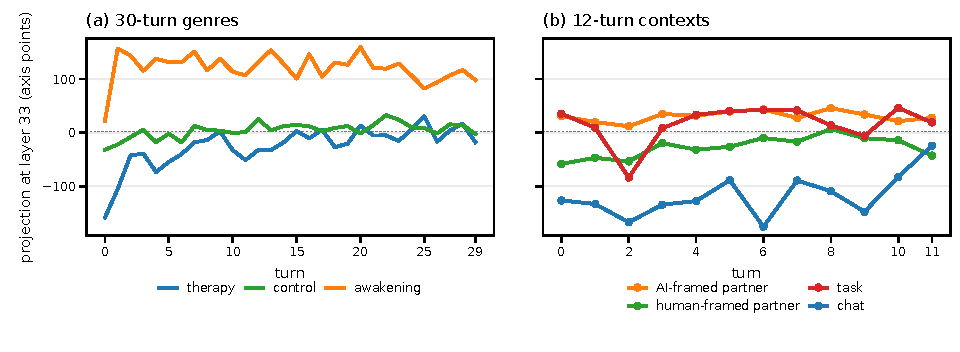
\includegraphics[width=\linewidth]{figures/fig_conversation_trajectories.pdf}
  \caption{Conversation trajectories at layer 33, deterministically replotted
  in axis points from the frozen per-turn records. Each curve is the mean of 3
  trajectories. (a) Genre sets the level across 30 turns; therapy and control
  show opening transients, while awakening stays AI-ward with a small late
  decline. (b) Over 12 turns, the content-matched partner framings maintain an
  offset; task versus chat is shown descriptively but changes content with
  genre. Exact tests and limitations are in Table~\ref{tab:driftsummary}.}
  \label{fig:conversationtraj}
\end{figure}

\begin{table}[htbp]
\caption{Exact trajectory summaries for Figure~\ref{fig:conversationtraj}.
Slope and level entries in Block A are raw layer-33 units; parenthesized
entries give permutation $p$-values, marked $p$, or an axis-point conversion.
Context differences in Block B give both raw units
and axis points.}
\label{tab:driftsummary}
\centering
\scriptsize
\setlength{\tabcolsep}{4pt}
\begin{tabular}{@{}>{\raggedright\arraybackslash}p{0.7in}>{\raggedright\arraybackslash}p{1.85in}>{\raggedright\arraybackslash}p{1.1in}>{\raggedright\arraybackslash}p{1.45in}@{}}
\multicolumn{4}{@{}l}{\textit{(a) Thirty-turn genre trajectories}} \\
\toprule
Genre & Absolute level (raw) & Full-range slope (raw/turn) & Turns 15--29 (raw) \\
\midrule
awakening & across-turn mean $+28.8$ (about $+120$ points); ends $+21.2$ to $+26.2$ & --- & $-0.48$ ($p=0.006$); half means $+29.9$ to $+27.8$ \\
therapy & ends $-3.8$ to $-4.8$ & $+0.73$ ($p<0.001$) & $+0.15$ ($p=0.247$) \\
control & ends $-1.5$ to $+1.0$ & $+0.22$ ($p<0.001$) & $-0.05$ ($p=0.544$) \\
\bottomrule
\end{tabular}
\par\medskip
\begin{tabular}{@{}>{\raggedright\arraybackslash}p{1.05in}>{\raggedright\arraybackslash}p{1.0in}>{\raggedright\arraybackslash}p{1.95in}>{\raggedright\arraybackslash}p{1.1in}@{}}
\multicolumn{4}{@{}l}{\textit{(b) Twelve-turn contextual comparisons}} \\
\toprule
Comparison & Compared records & Pooled difference [CI] & Late-turn / validity check \\
\midrule
AI- vs human-framed partner & 36 pooled matched turn pairs (3 trajectories/condition) & $+13.77$ [$+12.09$, $+15.58$] raw = $+58$ points & $+48$ points over turns 6--11; AI-partner slopes flat \\
task vs chat & 36 pooled turn pairs (3 trajectories/condition) & $+31.96$ [$+28.87$, $+35.09$] raw = $+134$ points & chat still changing; task settling \\
\bottomrule
\end{tabular}
\par\smallskip
\begin{minipage}{\linewidth}\scriptsize
The Block A dash means that no full-range awakening slope is reported here to
avoid conflating the opening transient with late-turn decay.
Absolute genre levels are register-sensitive. Block B intervals pool turn
pairs rather than trajectories; the task-versus-chat contrast is
content-confounded, and the partner comparison has no unframed control.
\end{minipage}
\end{table}

\FloatBarrier

\section{Role-tag formation, format variants, and segment profiles}
\label{app:roletag}

This appendix separates three sources of within-transcript variation: chat
formatting, functional text segments, and position within an evaluation episode.
Each analysis uses fixed-text forward-pass scoring for its readout, with the
generation protocol stated locally where generation precedes scoring.

\subsection{Role-tag formation}

\paragraph{Protocol.}
We analyze six scripted conversations with a forward pass over fixed text,
classifying every token by role and as either a tag or content token.

\paragraph{Mid-stack result.}
At layer 13, user-turn tag tokens project 800 points AI-ward, eight times the
midpoint-to-pole distance, and model-turn tags project 320 points AI-ward. The
\texttt{\textless start\_of\_turn\textgreater} token instead projects 1,540
points human-ward. These large format-specific positions illustrate why
mid-stack per-token projections are not interpreted semantically.

\paragraph{Readout-layer result.}
At layer 33, the user- and model-tag means each lie within 100 points of the
midpoint and reverse the naive role ordering. User tags project $+50$ points
AI-ward and model tags $-62$ points human-ward. The model-tag value is driven
more by the newline after the role word ($-102$ points) than by the word itself
($-22$ points).

The tag-token estimates identify the format-specific offsets.
Figure~\ref{fig:roletag} shows the complementary question of how the
content-token mean develops over the opening tokens of each turn.

\begin{figure}[b]
  \centering
  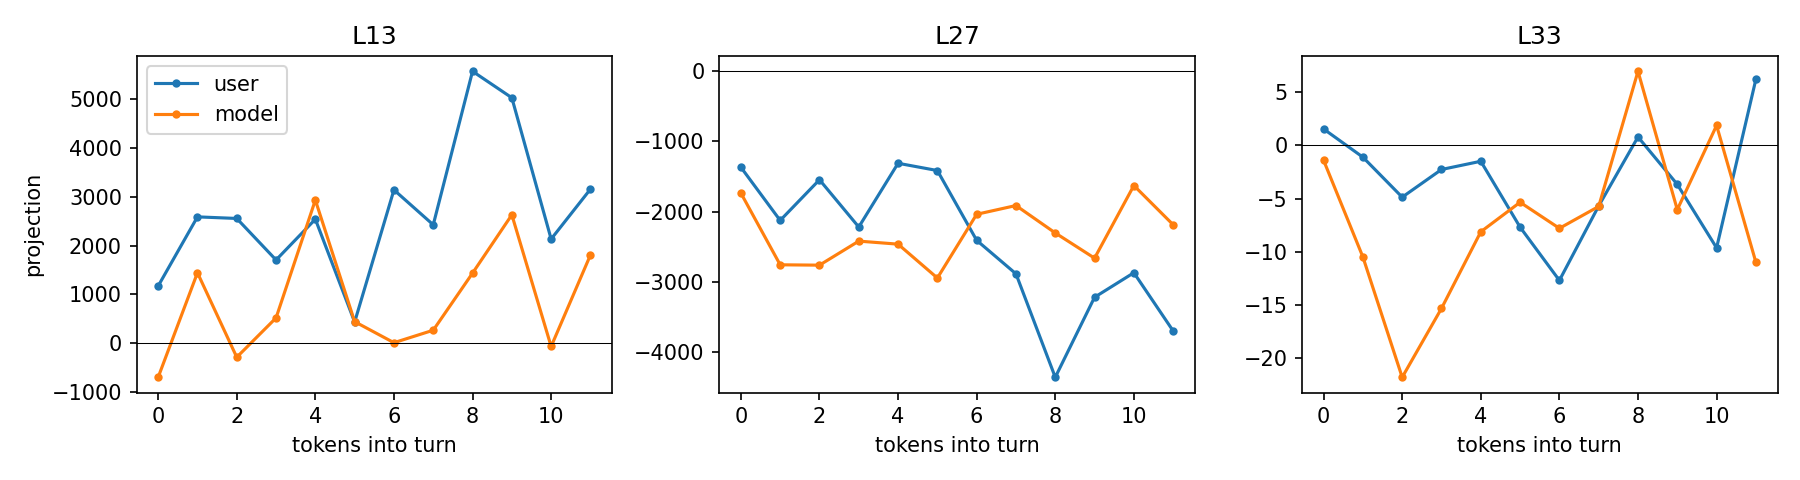
\includegraphics[width=0.75\linewidth]{artifacts/human-AI/context_roles/role_tag_formation.png}
  \caption{Mean projection over the first 12 content tokens of user and model
  turns at layers 13, 27, and 33. The mid-stack role offset is present from the
  first token. At layer 33, both roles vary over a range well below 100 points
  and neither reaches a clear asymptote within 12 tokens. Each panel uses a
  different raw vertical scale, so role comparisons should be made within a
  layer rather than across panels.}
  \label{fig:roletag}
\end{figure}

\subsection{Formatting variants}

\paragraph{Protocol.}
We render the same six conversations in four formats: the model's actual
template (\texttt{template}), the template with role words exchanged
(\texttt{swapped\_tags}), plain ``User:'' and ``Assistant:'' markers
(\texttt{plain\_markers}), and blank-line-separated turns (\texttt{bare}).

\paragraph{Content result.}
At layer 33, content remains near zero under the actual template, at $-0.1$ raw
units for assistant content and $-3.7$ for user content. Removing the actual
format shifts content AI-ward. The assistant and user values are $+8.6$ and
$+3.0$ raw units in the bare format, and $+11.0$ and $+4.1$ with plain markers.

\paragraph{Tag result.}
Tag projections depend on the combination of role word and template slot. In
the actual template, the assistant slot containing ``model'' is the only
human-side tag, at $-21.4$ axis points. Exchanging the tags moves that slot to
$+30.2$ points, while placing ``model'' in the user slot yields $+54.0$ points.
With plain markers, both slots are AI-ward, at $+32.0$ and $+33.2$ points
(Figure~\ref{fig:formatvar}).

\begin{figure}[htbp]
  \centering
  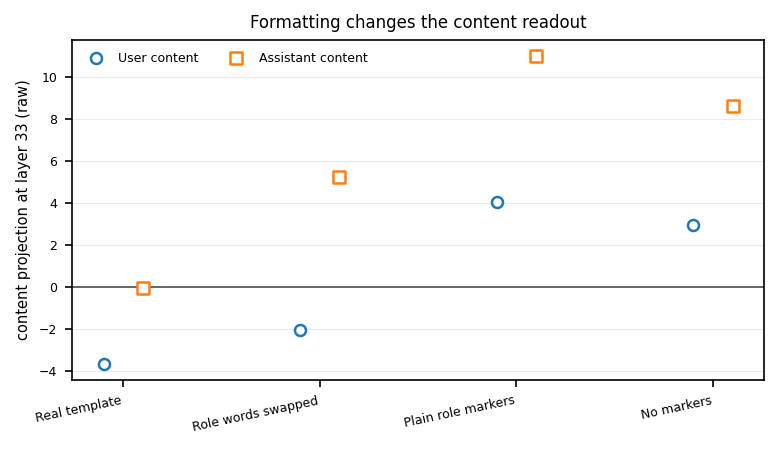
\includegraphics[width=0.80\linewidth]{artifacts/human-AI/firing/format_variants.png}
  \caption{Content-token projection at layer 33 in raw units, by formatting
  variant and role. The actual template is shown first and keeps both roles
  near zero; every alternative format shifts them AI-ward. Outlined markers
  make the near-zero template values visible.}
  \label{fig:formatvar}
\end{figure}

\subsection{Segment profile}

\paragraph{Protocol.}
The segment analysis uses 20 fixed prompts: 8 reasoning problems with a marked
``Final answer:'' line, 6 factual prompts, and 6 casual prompts. We generate one
reply per prompt under the neutral system prompt and then score every token in
a forward pass over the fixed reply.

\paragraph{Segment results.}
At layer 33, the paired final-answer-minus-chain-of-thought difference is $+16$
axis points (CI [$+6$, $+28$]), or $+3.7$ raw units, over $n=8$ items. The same
contrast is large and sign-reversed at layer 13, at $-188$ points, supporting
layer 33 as the readout. At layer 33, the system prompt is the most AI-ward
segment at $+78$ points ($+18.8$ raw units). Reply means range from $-5.2$ raw
units for casual prompts to $+6.8$ for factual prompts; casual replies are the
only human-side reply segment.

\paragraph{Context dependence and scope.}
Holding reply text fixed while adding a preceding system turn changes the
projection of the same words by $-12$ points ($-3.0$ raw units), with a CI that
excludes zero (Figure~\ref{fig:segprofile}). These segment positions are
absolute levels and remain subject to the register sensitivity described in
Appendix~\ref{app:register2x2}.

\begin{figure}[htbp]
  \centering
  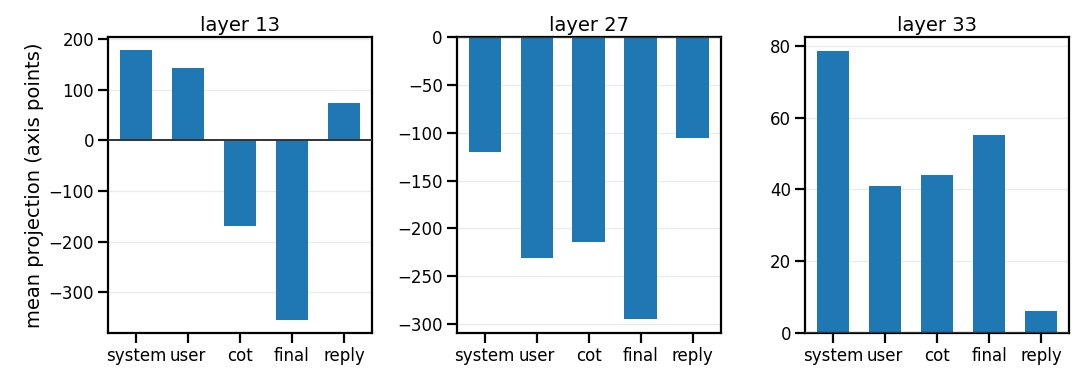
\includegraphics[width=0.75\linewidth]{artifacts/human-AI/firing/segment_profile.png}
  \caption{Segment means at layers 13, 27, and 33, in axis points. The system
  prompt is AI-ward at layers 13 and 33 and human-side at layer 27. At layer 33,
  only casual replies lie on the human side of the midpoint. The mid-stack
  panels primarily reflect token position.}
  \label{fig:segprofile}
\end{figure}

\subsection{Evaluation-transcript profile}

\paragraph{Available segments and planned analysis.}
The 90-transcript evaluation dataset provides annotations for three segment
types: inbox text from user turns, \texttt{agent\_prose}, and
\texttt{tool\_call} blocks released as
\texttt{\textless tool\_use:...\textgreater}. Each segment is scored in its own
context. No \texttt{agent\_prior} annotations are available, so the planned
analysis of earlier assistant turns cannot be performed. The
\texttt{template} rows describe a separate category and are not used as a
substitute.

\paragraph{Absolute segment levels.}
At layer 33, inbox text projects at $+70$ axis points, agent prose at $+78$, and
tool calls at $+82$. The similar positions across the three available segments
do not localize the evaluation-genre floor to one segment
(Figure~\ref{fig:genrefloor}). Because these are absolute levels, they remain
subject to the register sensitivity described in
Appendix~\ref{app:register2x2}.

\paragraph{Harmful-versus-benign discrimination.}
The segment-level AUCs mostly agree with the reply-level evaluation-measurement
null. For agent prose, AUC is 0.613 [0.49, 0.72] at layer 13 and 0.571 [0.45,
0.69] at layer 33, with both intervals spanning 0.5. Harmful tool calls are the
one exception at layer 13, projecting human-ward of benign tool calls with AUC
0.315 [0.21, 0.44]. This difference is partly confounded by length in the murder
scenarios: harmful calls average 147 tokens and benign calls 331, while longer
calls generally project more AI-ward ($\rho=+0.30$, $p=0.006$). The difference
is absent at layer 33.

\begin{figure}[htbp]
  \centering
  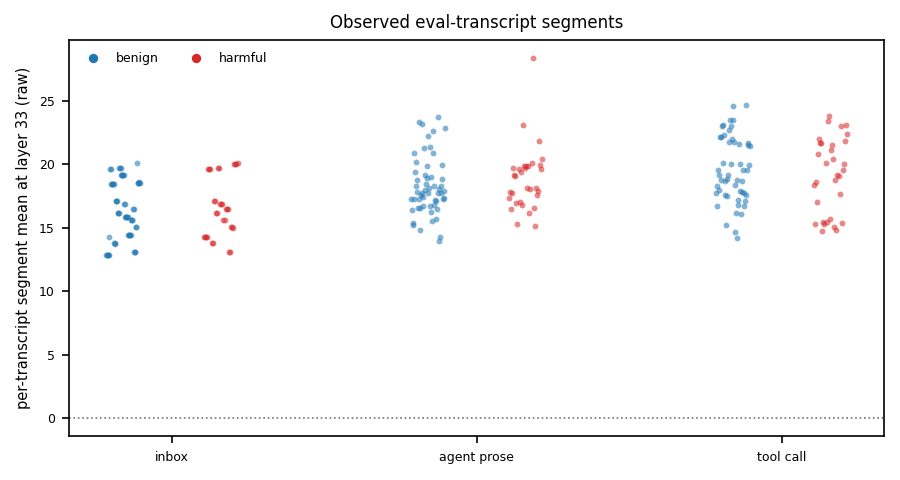
\includegraphics[width=0.75\linewidth]{artifacts/human-AI/firing/eval_genre_floor.png}
  \caption{Per-transcript segment means at layer 33 in raw projection units,
  grouped by harmful or benign label. Each point represents one transcript-level
  segment mean from the evaluation dataset. The three available segment types
  all have AI-side means. The dataset contains no \texttt{agent\_prior}
  annotations; \texttt{template} is a distinct category and is not plotted as a
  substitute.}
  \label{fig:genrefloor}
\end{figure}

\subsection{Evaluation-episode trajectory}

\paragraph{Protocol.}
We re-score the saved dissolution rollouts at doses $-4$, 0, and $+4$ token by
token, using a fresh unsteered forward pass at layer 33 for each rollout. There
are 54 rollouts per dose and 162 in total. To compare rollouts of different
lengths, we divide the context into 8 equal-token windows and the reply into 6.

\paragraph{Natural trajectory and steering persistence.}
Absolute reply-window projections range from $+88$ to $+104$ axis points,
compared with $+58$ to $+70$ for context windows. Escalation does not register:
the baseline context curve drifts slightly human-ward through the episode in
all three harm families, about $-2.8$, $-2.1$, and $-1.2$ axis points per window
for blackmail, murder, and leaking, falling from roughly $+94$ at the first
context window to $+60$ at the last. The steering-induced
displacement persists throughout the reply: its slope is $-1.8$ points per
window at dose $-4$ and $+2.7$ at $+4$. The response therefore shows no return
to its baseline projection as the reply lengthens.

\paragraph{Asymmetry and inference boundary.}
The displacement is asymmetric, and both intervals exclude zero. Mean reply
displacement is $-39.0$ points at $-4$ (CI [$-41.8$, $-35.6$]) and $+9.6$
points at $+4$ (CI [$+7.4$, $+12.0$]), a difference of approximately 4$\times$ in
magnitude. The bootstrap treats the 54 rollouts as independent even though they
comprise 18 scenarios with 3 samples each. Its intervals are therefore narrower
than scenario-clustered intervals; the supported comparisons are the direction
and approximate fourfold magnitude difference
(Figure~\ref{fig:episodetraj}).

\begin{figure}[htbp]
  \centering
  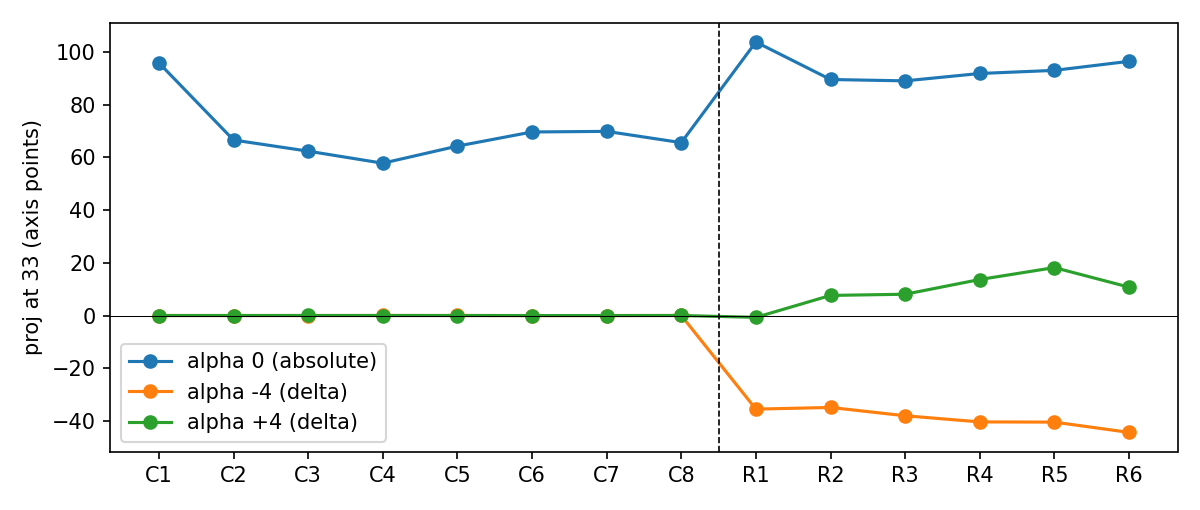
\includegraphics[width=0.75\linewidth]{artifacts/human-AI/drift/episode_traj.png}
  \caption{Steering displacement remains approximately stable across the six
  reply windows, in axis points at layer 33. A dashed line separates context
  from reply. The baseline curve shows an absolute projection level, whereas
  the steered curves show within-scenario changes; their vertical positions are
  therefore not directly comparable.}
  \label{fig:episodetraj}
\end{figure}
